\chapter{Il metodo di Denavit-Hartenberg}
Il metodo di \emph{Denavit-Hartemberg}, brevemente indicato con \emph{D-H}, è il più diffuso per la descrizione cinematica di meccanismi a catena aperta semplice (robot seriali). Il metodo può comunque essere utilizzato anche per meccanismi a catena chiusa ma non tratteremo questa sua possibile applicazione.

\paragraph{}
Dato un meccanismo seriale, il metodo permette di fissare in modo sistematico delle terne di riferimento su ognuno dei membri che compongono il meccanismo (dal telaio fino all’organo terminale che sia  pinza, mano o utensile) e di ricavare le leggi di trasformazione di coordinate che legano tra loro due terne contigue.

\section{Rototraslazioni}
In generale, due terne $\langle0\rangle$, $\langle1\rangle$ hanno diversa orientazione e origine non coincidente.\\
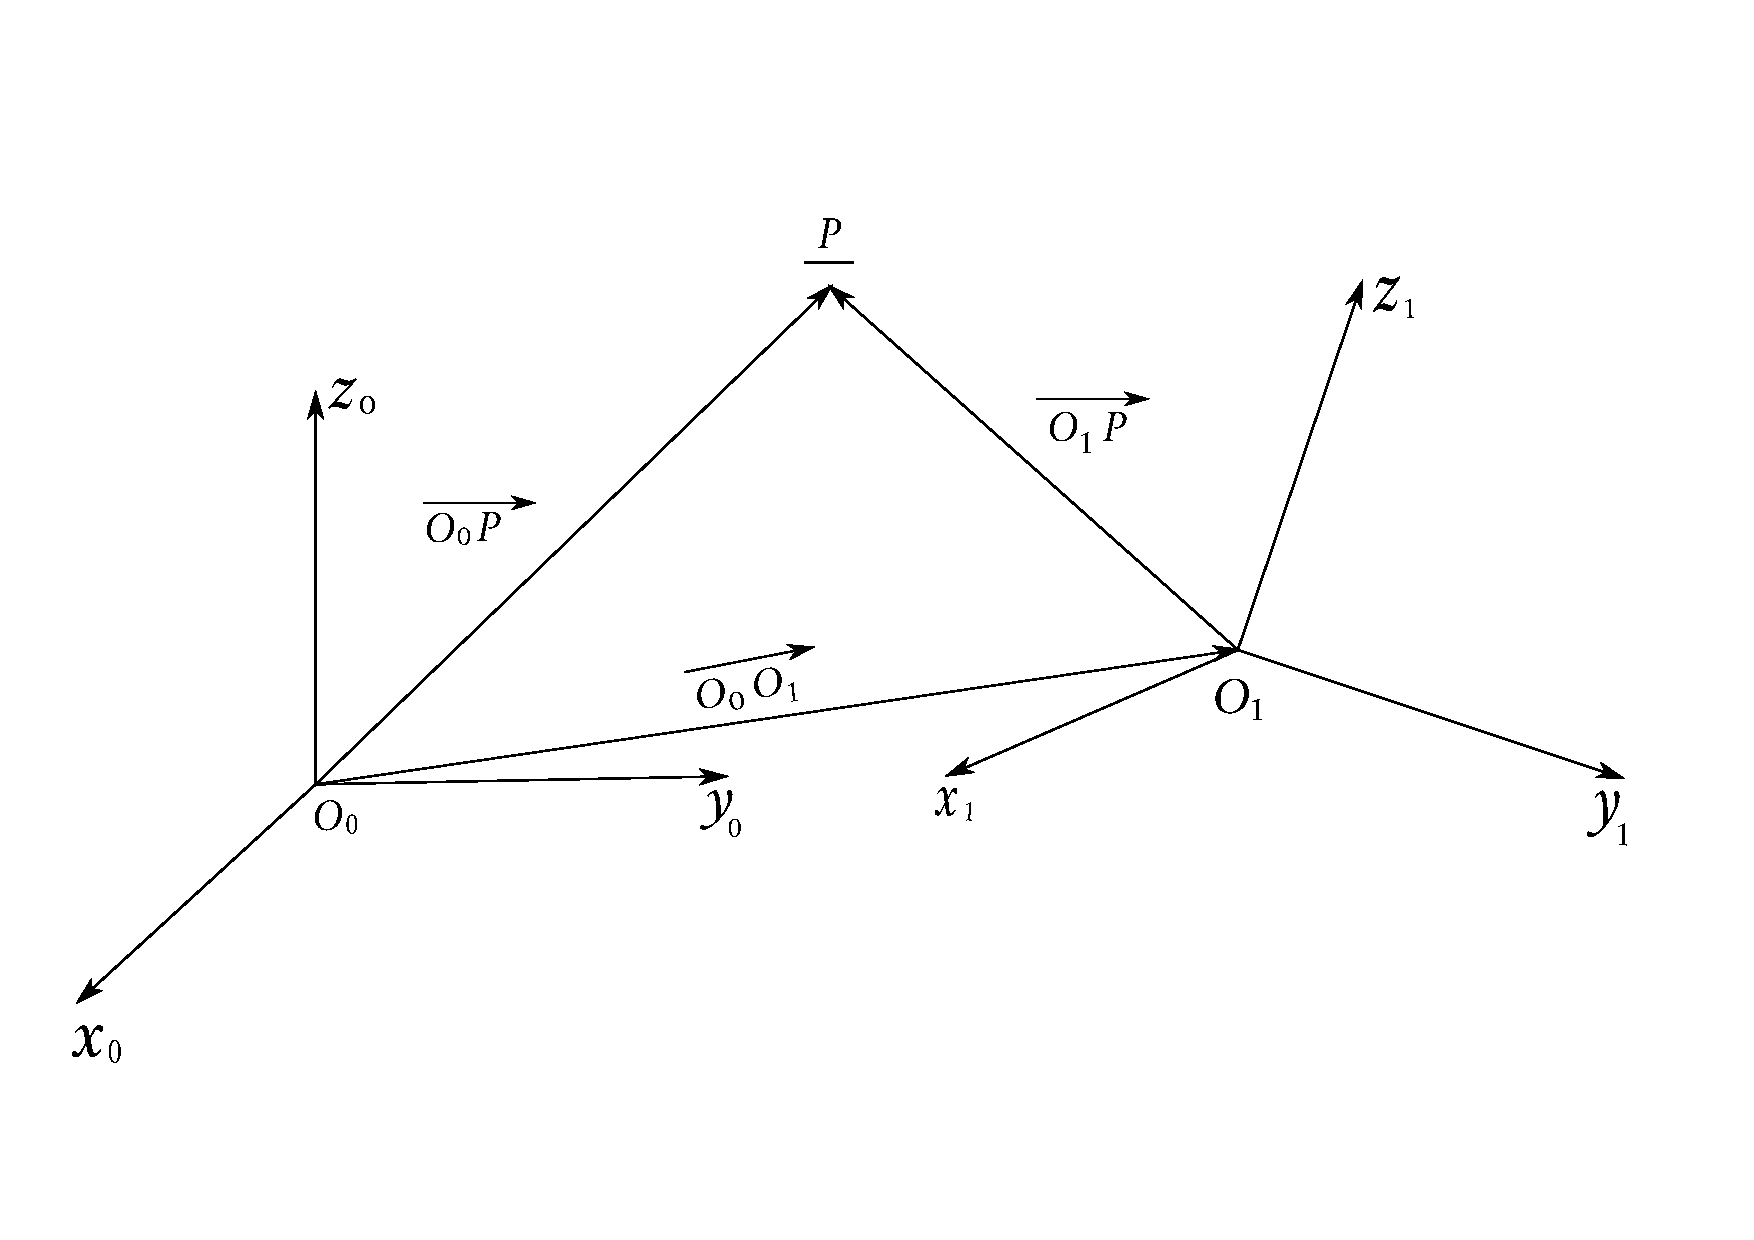
\includegraphics[scale=0.35]{rototraslazione.pdf}

Otteniamo, $\vec{O_{0}P} = \vec{O_0O_1} + \vec{O_1P}$, e scriviamo questa espressione in $\mathbb{R}^3$ con tutti i vettori riferiti alla terna $\langle0\rangle$: 
\begin{equation} \label{somma}
	^0\underline{P} = \,^0\underline{O_1} + R_1^0 \; ^1\underline{P} 
\end{equation}
L'operazione \eqref{somma} presenta una somma e una moltiplicazione, ma usande le \emph{coordinate omogenee}, l'equazione diventa una sola moltiplicazione.

\section{Coordinate Omogenee}
Per identificare un punto $\underline{P}$ nel piano si usano tre numeri $\underline{P}=
\begin{bmatrix}
	P_x & P_y & P_z
\end{bmatrix}^T$ 
e l'informazione contenuta in questi tre numeri può essere osservata anche se li moltiplichiamo per una costante arbitraria $\lambda \neq 0$ purchè si memorizzi la costante stessa. Pertanto il punto $\underline{P}$ possiamo rappresentarlo con quattro numeri nello spazio contenenti la stessa informazione della rappresentazione nel piano. Otteniamo:
\begin{equation}
	\underline{\tilde{P}} = 
	\begin{bmatrix}
		\lambda\underline{P} \\
		\lambda
	\end{bmatrix}
	=
	\begin{bmatrix}
		\lambda P_x \\
		\lambda P_y \\
		\lambda P_z \\
		\lambda
	\end{bmatrix}
\end{equation}
con $\underline{\tilde{P}}$ contenente la stessa informazione di $\underline{P}$. Nel seguito useremo sempre $\lambda = 1$.

\subsection{Trasformazioni omogenee}
Vediamo il \emph{cambio di coordinate} tra $\langle0\rangle$ e $\langle1\rangle$, con origine distinta, in \emph{coordinate omogenee}:
\begin{equation}
	\begin{cases}
		^0\underline{P} = R_1^0 \, ^1\underline{P} + \,^0\underline{O_1} = 			\begin{bmatrix}
			R_1^0 & ^0\underline{O_1}
		\end{bmatrix}
		\cdot
		\begin{bmatrix}
			^1\underline{P} \\
			1
		\end{bmatrix}\\
		1 = 
		\begin{bmatrix}
			0 & 0 & 0 & 1
		\end{bmatrix}
		\cdot
		\begin{bmatrix}
			^1\underline{P} \\
			1
		\end{bmatrix}
	\end{cases}
\end{equation}

ottenendo:
\begin{equation}
	\begin{bmatrix}
		^0\underline{P} \\
		1
	\end{bmatrix}
	=
	\begin{bmatrix}
		R_1^0 & ^0\underline{O_1} \\
		0\,0\,0 & 1
	\end{bmatrix}
	\begin{bmatrix}
		^1\underline{P} \\
		1
	\end{bmatrix}
	\Rightarrow
	\underline{^0\tilde{P}} = T_1^0 \; \underline{^1\tilde{P}}
\end{equation}

con:
\begin{equation} \label{trasformazione_omogenea}
	T_1^0 =
	\begin{bmatrix}
		R_1^0 & ^0\underline{O_1} \\
		0\,0\,0 & 1
	\end{bmatrix}
\end{equation}
$T_1^0$ della \eqref{trasformazione_omogenea} si dice \emph{matrice di trasformazione omogenea}, infatti, opera la trasformazione di coordinate omogenee di un punto tra due terne.
\subsection{Composizione di rototraslazioni successive}
Supponiamo di avere tre terne $\langle0\rangle$, $\langle1\rangle$, $\langle2\rangle$. Sia $T_1^0$ la matrice di trasformazione dalla terna $\langle0\rangle$ alla terna $\langle1\rangle$ e $T_2^1$ la matrice di trasformazione dalla terna $\langle1\rangle$ alla terna $\langle2\rangle$. Ci poniamo l'obiettivo di calcolare $T_2^0$. Per il generico punto $\underline{P}$, opportunamente riferito in coordinate omogenee rispetto alle tre terne, varranno le seguenti equazioni:
\begin{align} \label{p0} 
	^0\underline{\tilde{P}} = T_1^0 \, ^1\underline{\tilde{P}} \\
	\label{p1}
	^1\underline{\tilde{P}} = T_2^1 \, ^2\underline{\tilde{P}} \\
	^0\underline{\tilde{P}} = T_2^0 \, ^2\underline{\tilde{P}}
\end{align} 
Sostituendo l'espressione $^1\underline{\tilde{P}}$ della \eqref{p1} nella \eqref{p0}, otteniamo:
\begin{equation}
	^0\underline{\tilde{P}} =  T_1^0 \, T_2^1 \, ^2\underline{\tilde{P}}
\end{equation}
dovendo valere la (2.8) e la (2.9) per \emph{qualsiasi punto} $\underline{P}$, otterremo per $T_2^0$ la seguente espressione:
\begin{equation}
	T_2^0 = T_1^0 \; T_2^1
\end{equation}
\paragraph{}
Si generalizza a $n+1$ terne, ognuna mappata rispetto alla precedente da $T_{i}^{i-1}$, otteniamo:

\begin{equation}
	T_n^0 = T_1^0 \; T_2^1 \; \cdots \; T_{n-1}^{n-2} \; T_n^{n-1}
\end{equation}

\subsubsection{Calcolo rapido di $T_0^1$}
La matrice $T_0^1 = (T_1^0)^{-1}$ si può calcolare facendo l'inversa della \eqref{trasformazione_omogenea}, ma esiste un'altra strada più rapida, consideriamo $^0\underline{P} = R_1^0 \, ^1\underline{P} + \,^0\underline{O_1}$ e calcoliamo $^1\underline{P}$ da questa equazione:

\begin{equation*}
	^0\underline{P} = R_1^0 \; ^1\underline{P} + \,^0\underline{O_1} \Rightarrow R_1^0 \; ^1\underline{P} = \,^0\underline{P} - ^0\underline{O_1} \Rightarrow \,^1\underline{P} = (R_1^0)^T (^0\underline{P} - ^0\underline{O_1})
\end{equation*}
ottenendo:
\begin{equation*}
	\,^1\underline{P} = R_0^1 \; ^0\underline{P} - R_0^1 \; ^0\underline{O_1}
\end{equation*}
e pertanto otteniamo:
\begin{equation}
	T_0^1 =
	\begin{bmatrix}
		R_0^1 & -R_0^1 \; ^0\underline{O_1} \\
		0\,0\,0 & 1
	\end{bmatrix}
\end{equation}
\newpage
\section{Metodo di Denavit-Hartenberg}
Si tratta di un \emph{metodo sistematico} per descrivere catene cinematiche, ovvero, insiemi di corpi rigidi collegati tra loro da \emph{coppie cinematiche} rotoidali o prismatiche. Da qui in avanti le coppie cinematiche le chiameremo \emph{giunti}.

\subsection{Passi del metodo per grandi linee}
\begin{enumerate}
	\item Si numerano i membri (link), da $0$ a $n$.
	\item Si numerano i giunti, da $1$ a $n$.
	\item Si fissano, con alcune regole, $n+1$ terne ai vari link.
	\item Si calcola $T_i^{i-1}\quad\forall n$.
	\item Si ottiene $T_0^n = T_0^1\,T_2^1\,\cdots\,T_{n-1}^{n-2}\,T_n^{n-1}$
\end{enumerate}

Il metodo \emph{D-H} ci permette di ridurre da sei a quattro il numero di parametri necessari per costruire $T_i^{i-1}$, infatti, tre parametri saranno fissi ed uno sarà variabile (\emph{coordinata di giunto}).

\subsection{Regole generali per fissare la terna $i$ sul link $i$}
\begin{enumerate}
	\item[0.] Una volta numerati link e giunti
	\item[1.] L'asse $z_{i-1}$ si sceglie:
	\begin{itemize}
		\item Coincidente con l'asse di rotazione del giunto $i$ se questo è rotoidale, scegliendo il verso con buonsenso.
		\item Parallelo alla direzione di moto del giunto $i$ se questo è prismatico.
	\end{itemize}
	notiamo che l'asse $z_n$ è arbitrario e quindi lo possiamo scegliere con "buonsenso".
	\item[2.]In generale si sceglie l'asse $x_i$ come la retta di minima distanza, orientata da $z_{i-1}$ a $z_i$. Questa regola ha dei casi particolari:
	\begin{itemize}
		\item Se non esiste l'asse $z_{i-1}$ allora non posso applicare la regola per fissare $x_0$, quindi fisso questo asse arbitrariamente con il vincolo $x_{0}\,\perp\,z_{0}$ così scegliamo anche $O_0$.
		\item Se $z_{i-1}\parallel z_i$ allora $x_i$ va scelto arbitrariamente pur facendo presente che il verso da $z_{i-1}$ a $z_i$ è definito.
		\item Se $z_{i-1}$ e $z_i$ sono \emph{incidenti} allora la retta di minima distanza degenera nella normale comune ed il verso di $x_i$ va scelto arbitrariamente tale che $\underline{i_i} = \pm \underline{k_{i-1}} \times \underline{k_i}$ e poniamo quindi il vincolo di ortogonalità dell'asse $x_i$ sia per $z_i$ che per $z_{i-1}$.
	\end{itemize}
\end{enumerate}

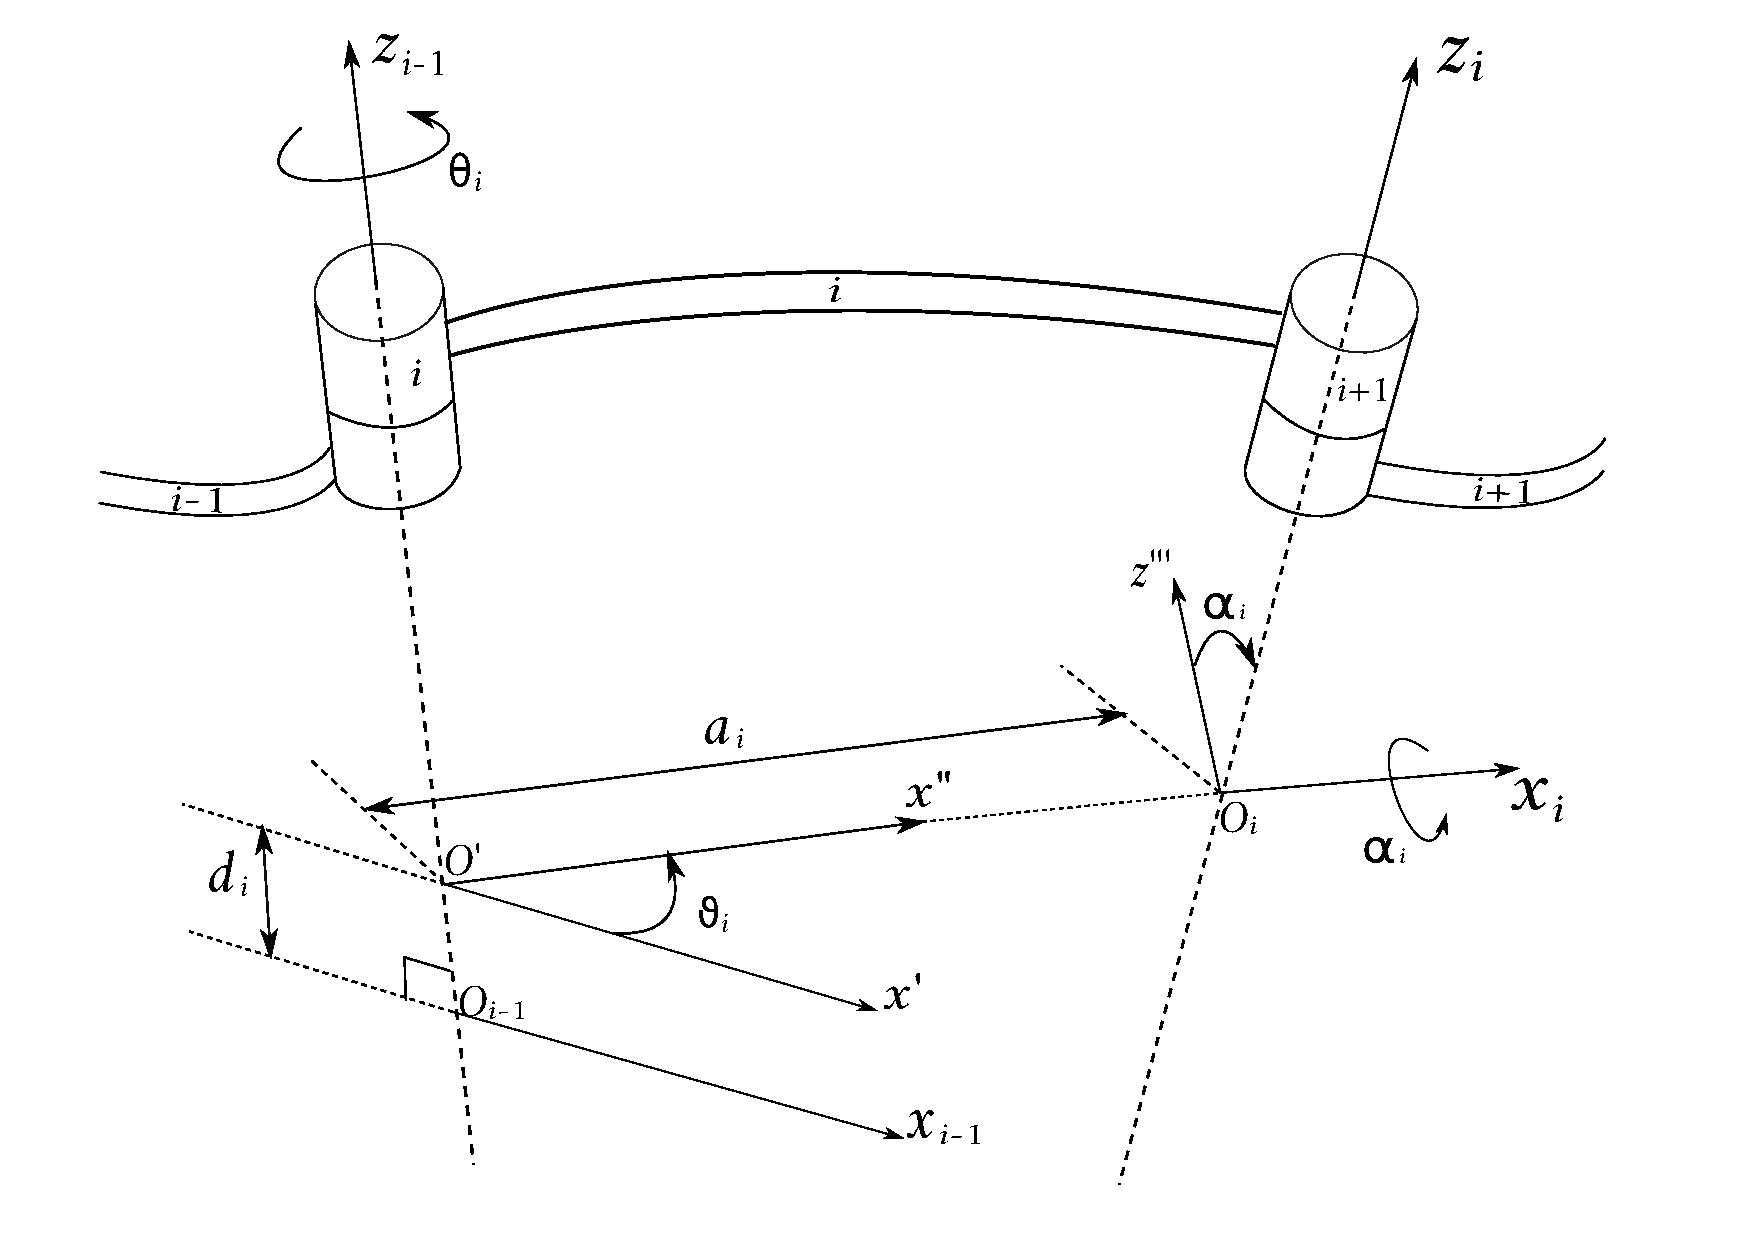
\includegraphics[scale=0.4]{metodoDH.pdf}
\captionof{figure}{Terne e trasformazioni nel metodo D-H}

\subsection{Calcolo di $T_i^{i-1}$}
Per ottenere $T_i^{i-1}$ scomponiamola in quattro trasformazioni successive specificate in terna corrente che portino $\langle i-1 \rangle$ a sovrapporsi alla terna $\langle i \rangle$:
\begin{enumerate}
	\item Trasformazione lungo $z_{i-1}$ di una quantità $d_{i}\gtreqless0$, fino a che l'origine della terna corrente non si sposta in $O'\,\in\,x_i$.
	\item Rotazione attorno a $z_{i-1}$ di un angolo $\theta_{i}\lesseqgtr0$, fino a che l'asse $x$ della terna corrente non si allinea con $x_i$.
	\item Traslazione lungo $x_i$ di una quantità $a_{i}\geqslant0$ (lunghezza del segmento di minima distanza tra $z_{i-1}$ e $z_i$), fino a che l'origine non va a coincidere con $O_i$.
	\item Rotazione attorno a $x_i$ di un angolo $\alpha_{i}\lesseqgtr0$, fino a che la terna corrente non è allineata con la terna $<i>$.
\end{enumerate}
Notiamo che $\alpha_i$ e $a_i$ sono sempre fissi, $d_i$ è variabile se il giunto $i$ è prismatico e $\theta_i$ è variabile se il giunto $i$ è rotoidale.

\paragraph{}
Vediamo le quattro trasformazioni:
\begin{equation*}
	1) =
	\begin{bmatrix}
		1 & 0 & 0 & 0 \\
		0 & 1 & 0 & 0 \\
		0 & 0 & 1 & d_i \\
		0 & 0 & 0 & 1
	\end{bmatrix}
	\quad 2) =
	\begin{bmatrix}
		C_{\theta_i} & -S_{\theta_i} & 0 & 0 \\
		S_{\theta_i} & C_{\theta_i} & 0 & 0 \\
		0 & 0 & 1 & 0 \\
		0 & 0 & 0 & 1
	\end{bmatrix}
\end{equation*}
\begin{equation*}
	3) =
	\begin{bmatrix}
		1 & 0 & 0 & a_i \\
		0 & 1 & 0 & 0 \\
		0 & 0 & 1 & 0 \\
		0 & 0 & 0 & 1
	\end{bmatrix}
	\quad 4) =
	\begin{bmatrix}
		1 & 0 & 0 & 0 \\
		0 & C_{\alpha_i} & -S_{\alpha_i} & 0 \\
		0 & S_{\alpha_i} & C_{\alpha_i} & 0 \\
		0 & 0 & 0 & 1
	\end{bmatrix}
\end{equation*}
a questo punto facendo il prodotto otteniamo,
\begin{equation*}
	1)\cdot2) =
	\begin{bmatrix}
		C_{\theta_i} & -S_{\theta_i} & 0 & 0 \\
		S_{\theta_i} & C_{\theta_i} & 0 & 0 \\
		0 & 0 & 1 & d_i \\
		0 & 0 & 0 & 1
	\end{bmatrix}
	\quad 3)\cdot4) =
	\begin{bmatrix}
		1 & 0 & 0 & a_i \\
		0 & C_{\alpha_i} & -S_{\alpha_i} & 0 \\
		0 & S_{\alpha_i} & C_{\alpha_i} & 0 \\
		0 & 0 & 0 & 1
	\end{bmatrix}
\end{equation*}
e facendo il prodotto tra queste due matrici otteniamo la \emph{matrice di trasformazione complessiva} $T_i^{i-1}$:
\begin{equation}
	T_i^{i-1} = 
	\begin{bmatrix}
		C_{\theta_i} & -C_{\alpha_i}\,S_{\theta_i} & S_{\alpha_i}\,S_{\theta_i} & a_i\,C_{\theta_i} \\
		S_{\theta_i} & C_{\alpha_i}\,C_{\theta_i} & -S_{\alpha_i}\,C_{\theta_i} & a_i\,S_{\theta_i} \\
		0 & S_{\alpha_i} & C_{\alpha_i} & d_i \\
		0 & 0 & 0 & 1
	\end{bmatrix}
\end{equation}

\subsubsection{Esercizio:}
Consideriamo un manipolatore planare $3R$ (tre giunti rotoidali) e applichiamo il metodo $D-H$.

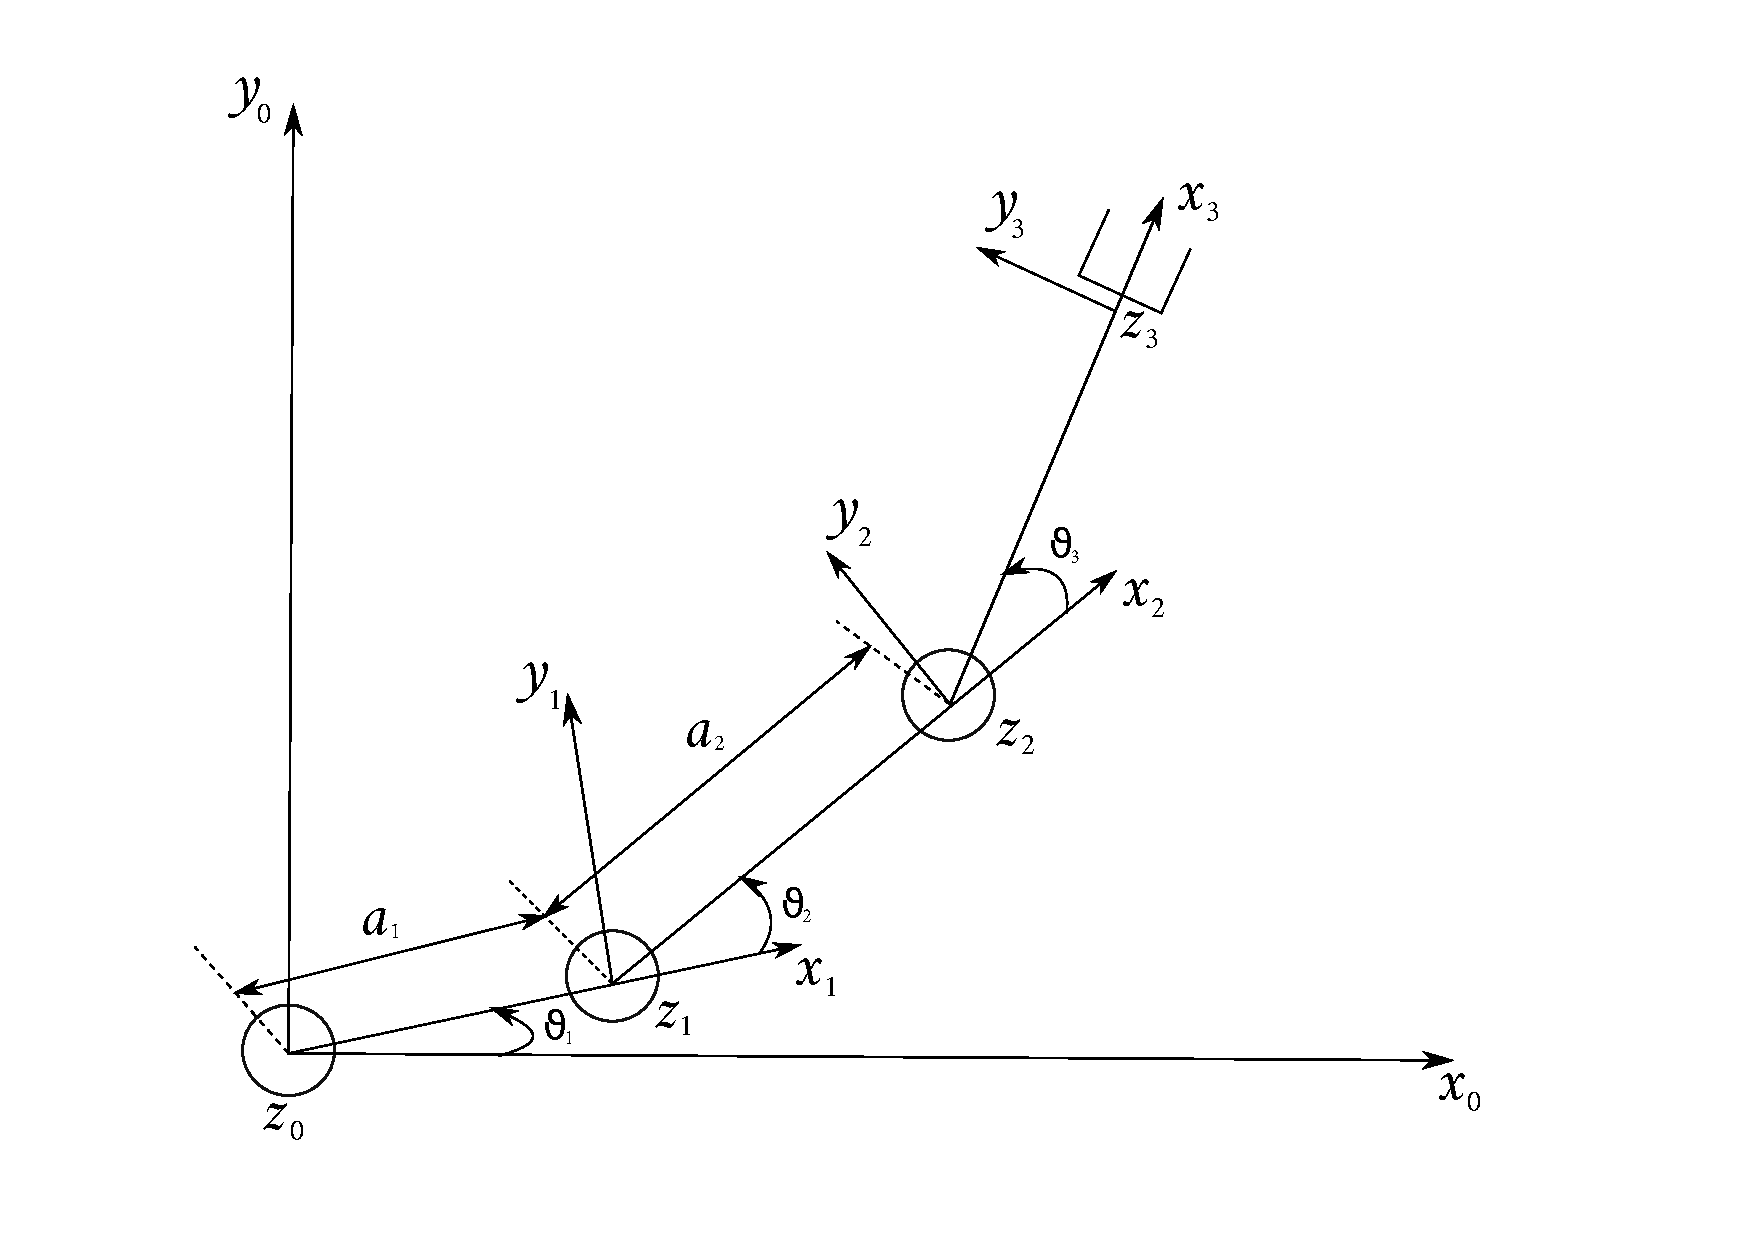
\includegraphics[scale=0.4]{manipolatore3R.pdf}
\captionof{figure}{Manipolatore planare a 3 gradi di libertà, schema cinematico}

Scriviamo la tabella $D-H$:\\
\begin{center}
$
\begin{array}{ccccc}
\toprule
Giunti & d_1 & \theta_i & a_i & \alpha_i \\
\midrule
1 & 0 & q_1 & l_1 & 0 \\
2 & 0 & q_2 & l_2 & 0 \\
3 & 0 & q_3 & l_3 & 0 \\
\bottomrule
\end{array}
$
\end{center}

\paragraph{}
Abbiamo tre modi di procedere:
\begin{itemize}
	\item Metodo sistematico: dalla tabella calcolo $T_1^0$, $T_2^1$, $T_3^2$ e poi le moltiplico.
	\item Metodo intermedio: scrivo "a occhio" le tre matrici e le moltiplico.
	\item Metodo geometrico: in questo caso ho meno calcoli.
\end{itemize}

Otteniamo:
\begin{equation}
	T_3^0 = 
	\begin{bmatrix}
		C_{123} & -S_{123} & 0 & a_1\,C_{\theta_i}+a_2\,C_{12}+ a_3\,C_{123} \\
		S_{123} & C_{123} & 0 & a_1\,S_{\theta_i}+a_2\,S_{12}+ a_3\,S_{123} \\
		0 & 0 & 1 & 0 \\
		0 & 0 & 0 & 1 \\
	\end{bmatrix}
\end{equation}
con: $C_{12} = \cos(\theta_1 + \theta_2)$ e $C_{123} = \cos(\theta_1 + \theta_2 + \theta_3)$.

\section{Manipolatore Antropomorfo}
Applichiamo il metodo \emph{D-H} ad un robot a tre gradi di libertà (\emph{DOF, Degree of Freedom}). Questo manipolatore prende il nome di \emph{antropomorfo} perchè ricorda un braccio umano. I membri sono numerati da $0$ a $3$. Sono presenti tre giunti rotoidali numerati da $1$ a $3$ con le seguenti proprietà:
\begin{itemize}
	\item $Giunto\, 1$: ha asse verticale.
	\item $Giunto\, 2 \,(spalla)$: ha asse orizzontale ed è ortogonale al giunto 1.
	\item $Giunto\, 3 \, (gomito)$: ha asse orizzontale ed è parallelo al giunto 2.
\end{itemize}

\begin{center}
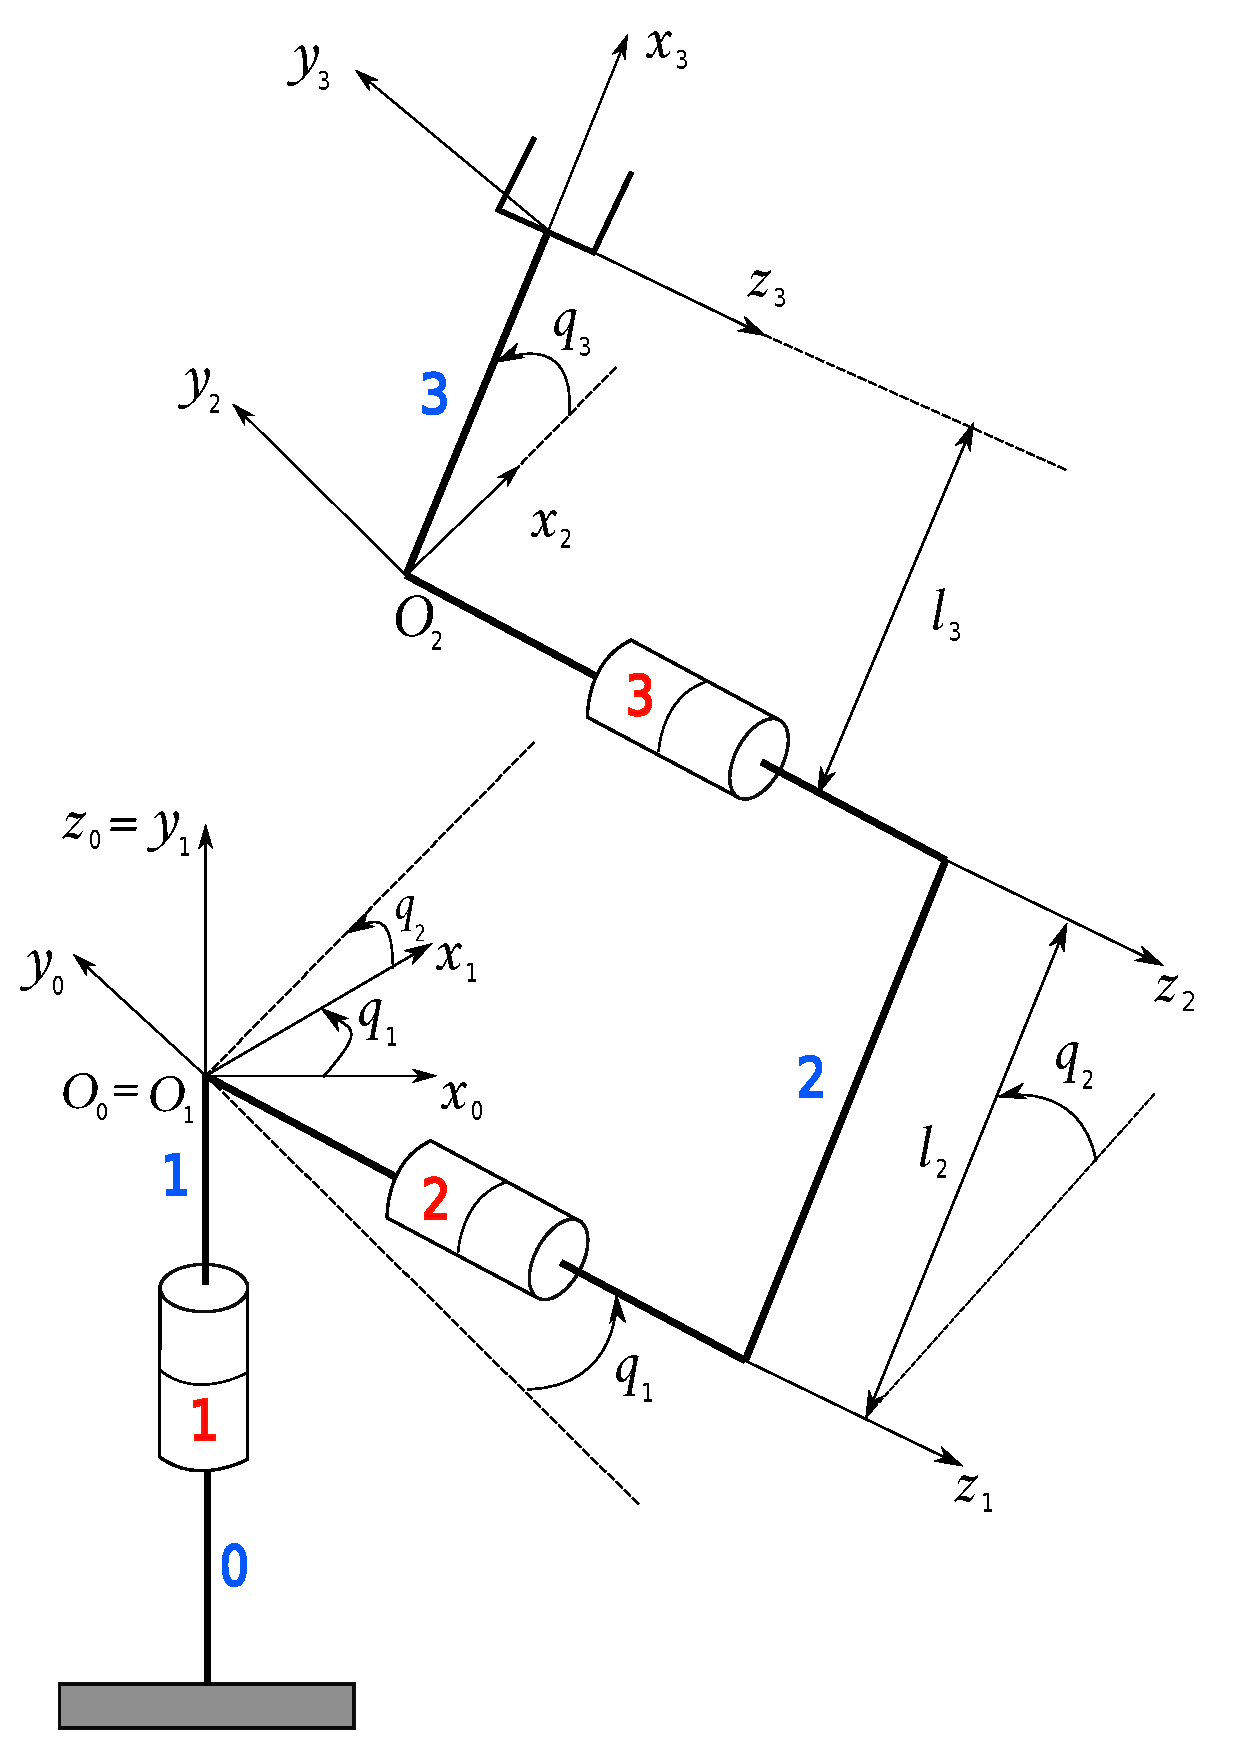
\includegraphics[scale=0.4]{manipolatoreAntropomorfo.pdf}
\captionof{figure}{Manipolatore Antropomorfo}
\end{center}

\subsubsection{Applicazione del metodo:}
Il metodo viene applicato nel modo seguente:
\begin{itemize}
	\item gli assi $z_0$, $z_1$, $z_2$ sono scelti coincidenti con gli assi dei $giunti \; 1,2,3$.
	\item l'asse $z_3$ è arbitrario e lo scegliamo parallelo agli assi $z_1$ e $z_2$
	\item l'asse $x_0$ è stato scelto ortogonale a $z_0$.
	\item gli assi $z_0$ e $z_1$ sono mutuamente ortogonali, l'asse $x_1$ è scelto in modo che $\underline{i_1} = \underline{k_0} \times \underline{k_1}$
	\item notiamo che $x_1$ sta nel piano $x_0y_0$, ovvero, piano orizzontale passante per $O_0$.
	\item dato che $z_1$ e $z_2$ sono paralleli, $x_2$ lo scegliamo passante per $O_1$
	\item scegliamo $x_3$ lungo la direzione di approccio della terna utensile
\end{itemize}


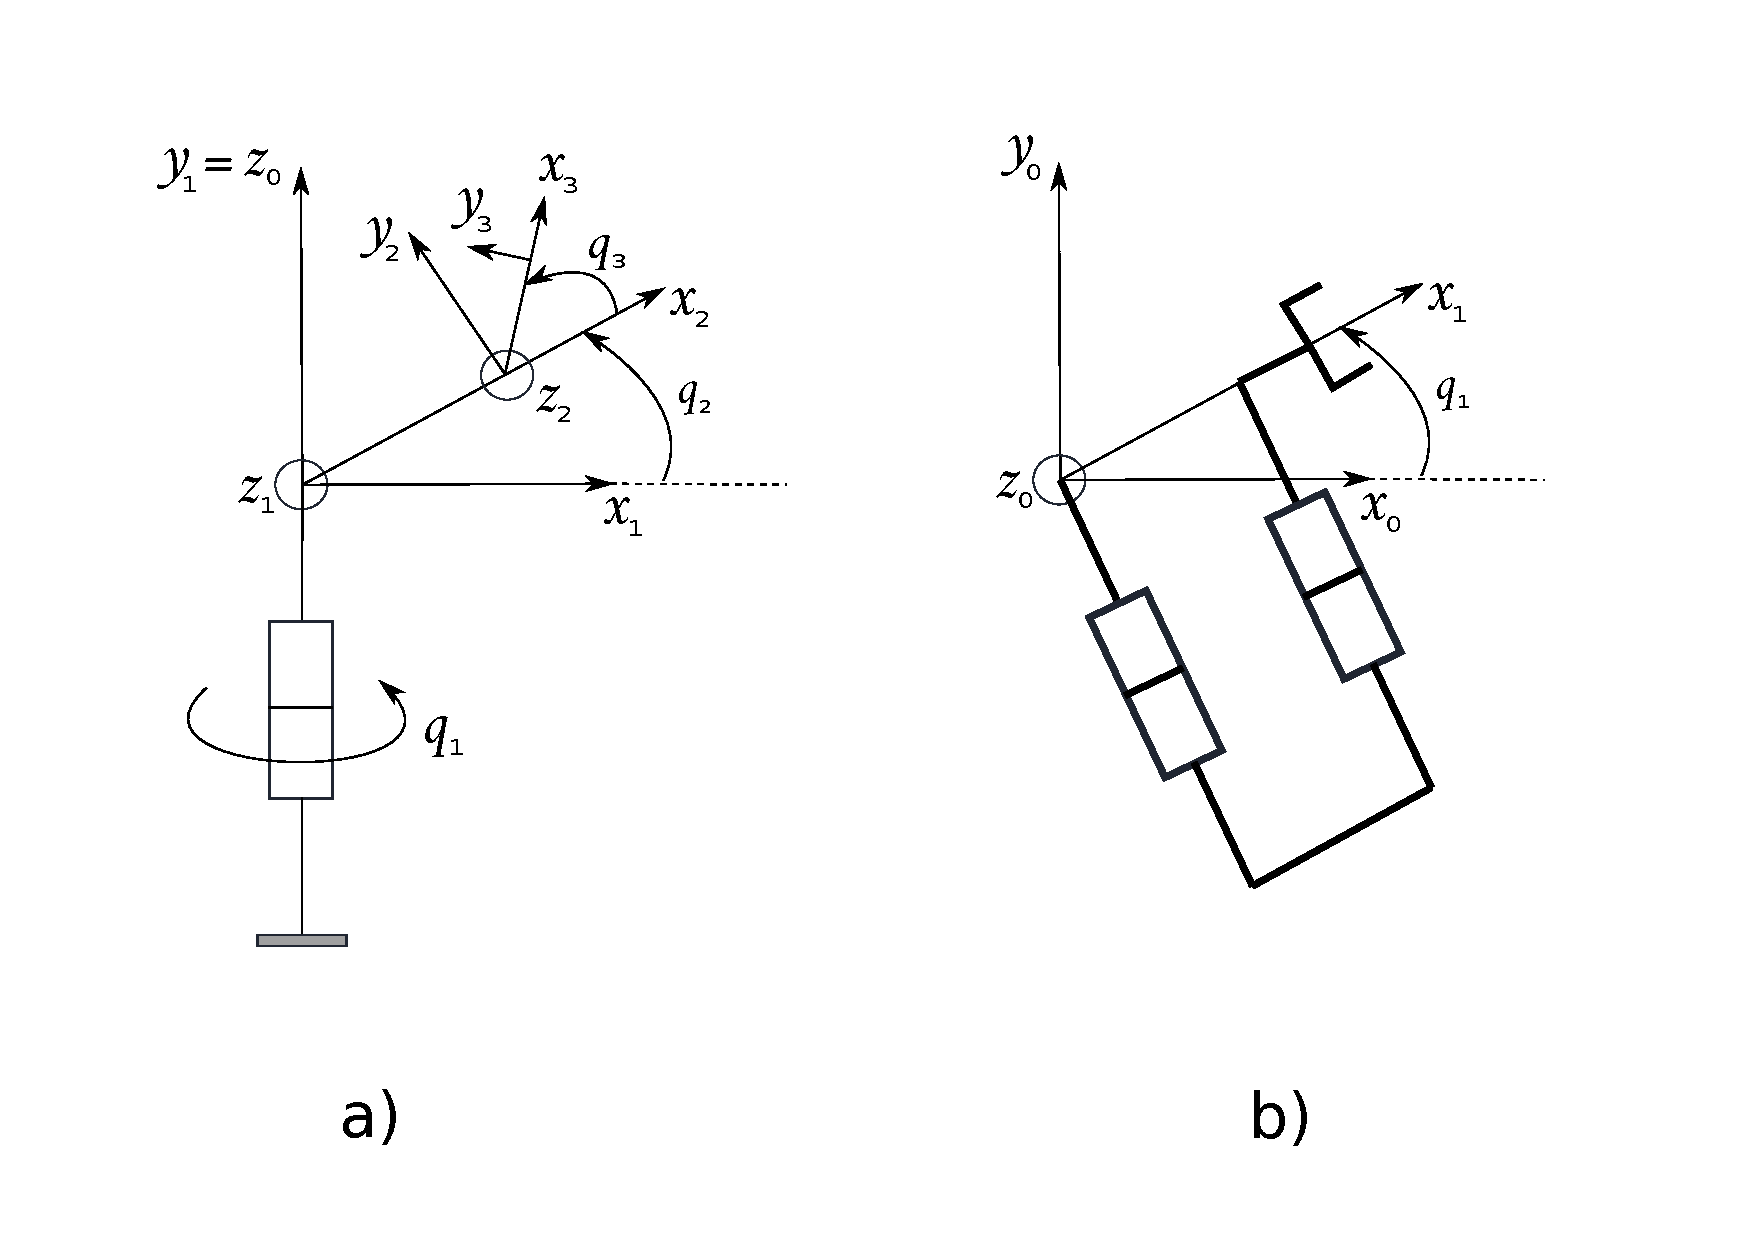
\includegraphics[scale=0.4]{visteManipolatore.pdf}
\captionof{figure}{a) vista da $z_1$  b) vista in pianta, proiezione su $x_0y_0$}

\subsubsection{Compiliamo la tabella $d_i, \theta_i, a_i, \alpha_i$:}
\begin{enumerate}
	\item $Giunto 1$:
	\begin{itemize}
		\item le origini delle terne $\langle0\rangle$ e $\langle1\rangle$ coincidono, quindi $d_1 = 0$
		\item l'asse $x_1$ si ottiene ruotando l'asse $x_0$ attorno all'asse $z_0$ di un angolo $q_1$, positivo se concorde con $z_0$
		\item la minima distanza tra $z_0$ e $z_1$ è zero, quindi $l_1 = 0$
		\item l'asse $z_1$ si ottiene ruotando l'asse $z_0$ attorno a $x_1$ di $90$, quindi $\alpha_1 = 90$
	\end{itemize}
	\item $Giunto 2$:
	\begin{itemize}
		\item $O_1$ si trova già sull'asse, quindi $d_2 = 0$
		\item l'asse $x_2$ forma rispetto all'asse $x_1$ un angolo $q_2$
		\item la minima distanza tra $z_1$ e $z_2$ è pari ad $l_1$
		\item l'asse $z_2$ è parallelo all'asse $z_1$, quindi $\alpha_2 = 0$
	\end{itemize}
	\item $Giunto 3$:
	La trasformazione dalla terna $\langle2\rangle$ alla terna $\langle3\rangle$ è sostanzialmente identica a quella dalla $\langle1\rangle$ alla $\langle2\rangle$, quindi $d_3 = 0$, $\theta_3 = q_3$ la distanza tra gli assi $z_2$ e $z_3$ è pari ad $l_3$ e $\alpha_3 = 0$.
\end{enumerate}
La tabella risulta:
\begin{center}
$
\begin{array}{|c|c|c|c|c|}
\toprule
Giunti & d_i & \theta_i & a_i & \alpha_i \\
\midrule
1 & 0 & q_1 & 0 & 90 \\
2 & 0 & q_2 & l_2 & 0 \\
3 & 0 & q_3 & l_3 & 0 \\
\bottomrule
\end{array}
$
\end{center}


\section{Polso Sferico}
Il polso sferico \emph{roll-pitch-roll} possiede 3 giunti rotoidali i cui assi si intersecano in un punto detto \emph{"centro del polso"}. 

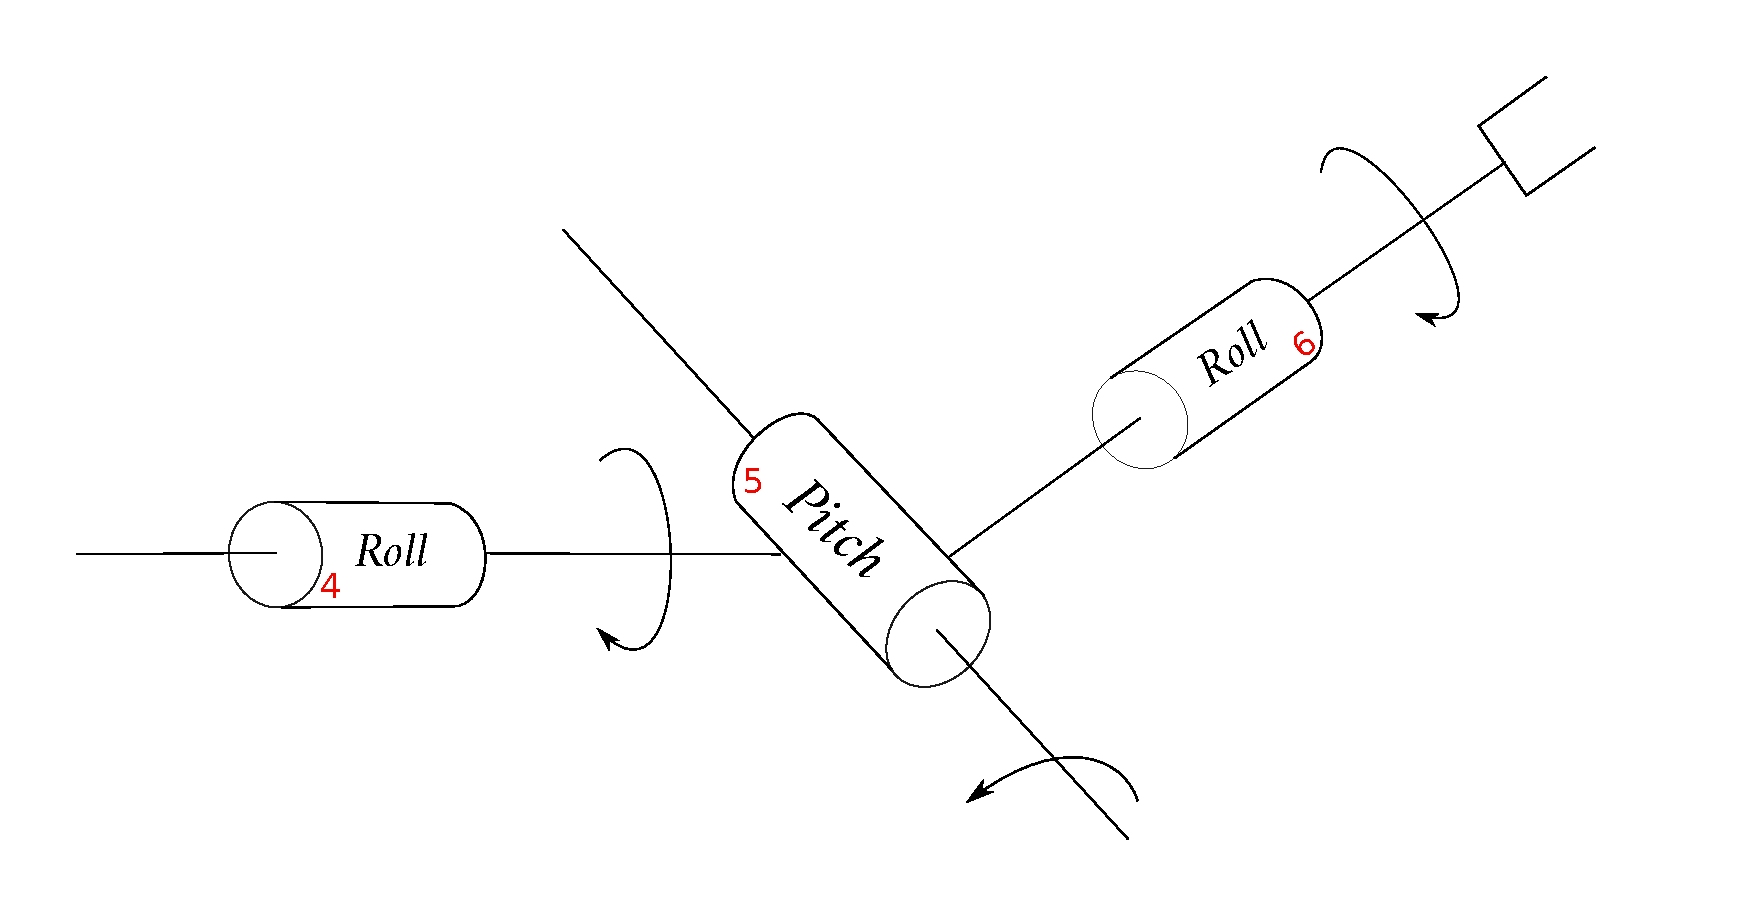
\includegraphics[scale=0.4]{polsoSferico.pdf}
\captionof{figure}{Polso sferico \emph{roll-pitch-roll}}

Esso viene utilizzato per \emph{completare} la struttura cinematica di un manipolatore a 3 DOF (che sia cilindrico, sferico o antropomorfo), consentendo di ottenere l'orientazione desiderata dell'organo terminale. Pertanto numeriamo i giunti $4$, $5$, $6$. 

\paragraph{}
Per capire la geometria del polso, disegniamolo in \emph{configurazione singolare}, ovvero con gli assi $z_3 \parallel z_5$ e notiamo:
\begin{itemize}
	\item $x_3$ normale comune a $z_2z_3$
	\item $x_4$ normale comune a $z_3z_4$
	\item $x_5$ normale comune a $z_4z_5$
	\item $x_6$ ortogonale al piano della pinza, quindi a $z_6$ 
\end{itemize}

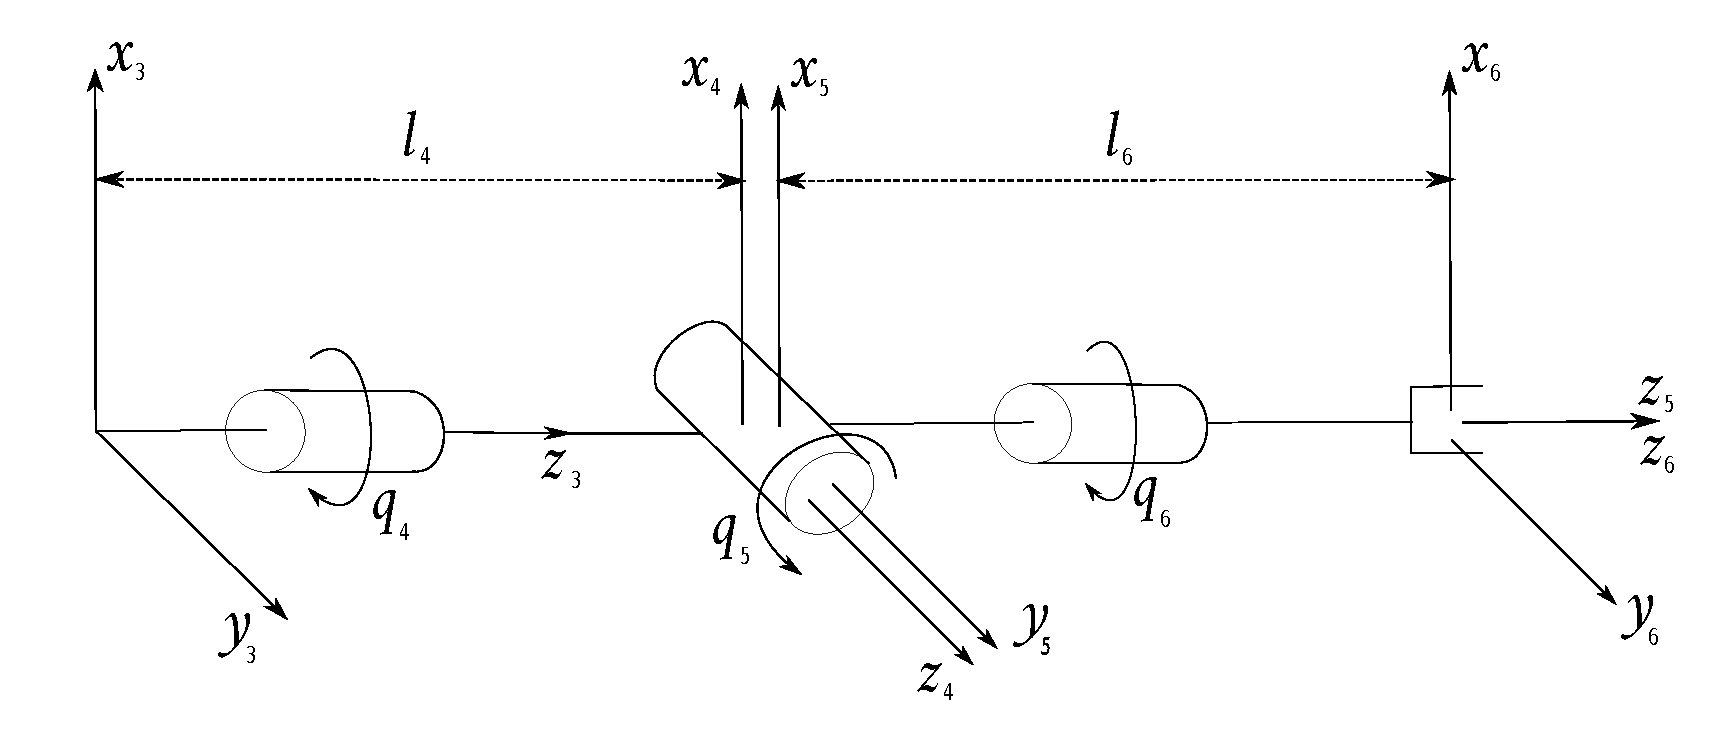
\includegraphics[scale=0.4]{polsoSfericoSingolare.pdf}
\captionof{figure}{Configurazione Singolare del polso.}

\paragraph{}
La tabella $D-H$ risulta:
\begin{center}
$
\begin{array}{ccccc}
\toprule
Giunti & d_1 & \theta_i & a_i & \alpha_i \\
\midrule
4 & l_4 & q_4 & 0 & -90 \\
5 & 0 & q_5 & 0 & 90 \\
6 & l_6 & q_6 & 0 & 0 \\
\bottomrule
\end{array}
$
\end{center}

\paragraph{}
A questo punto calcoliamo $T_i^{i-1}(d_i, \theta_i, a_i, \alpha_i)$, ovvero $T_4^3$, $T_5^4$, $T_6^5$ con \emph{intuito geometrico}. 

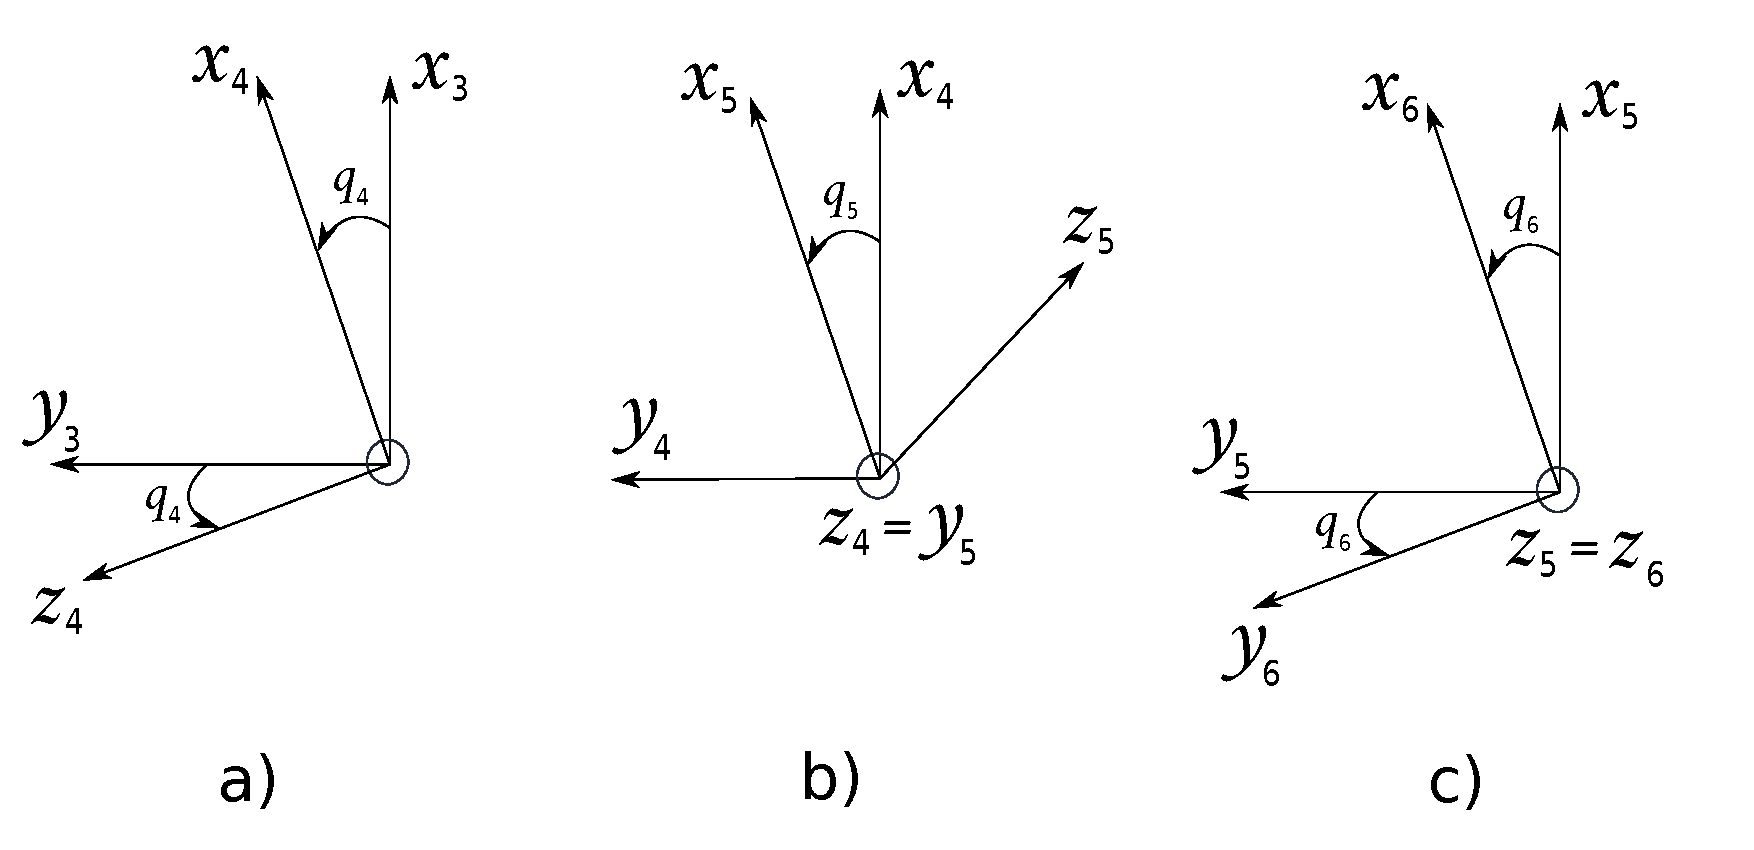
\includegraphics[scale=0.4]{polsoSfericoGeometria.pdf}
\captionof{figure}{a) vista da $z_3$ b) vista da $z_4$ c) vista da $z_5$}

\begin{equation}
	T_4^3 = 
	\begin{bmatrix}
		C_4 & 0 & -S_4 & 0 \\
		S_4 & 0 & C_4 & 0 \\
		0 & -1 & 0 & l_4 \\
		0 & 0 & 0 & 1 \\
	\end{bmatrix}
	\quad T_4^5 =
	\begin{bmatrix}
		C_5 & 0 & S_5 & 0 \\
		S_5 & 0 & -C_5 & 0 \\
		0 & 1 & 0 & 0 \\
		0 & 0 & 0 & 1 \\
	\end{bmatrix}
	\quad T_6^5 = 
	\begin{bmatrix}
		C_6 & -S_6 & 0 & 0 \\
		S_6 & C_6 & 0 & 0 \\
		0 & 0 & 1 & l_6 \\
		0 & 0 & 0 & 1 \\
	\end{bmatrix}
\end{equation}

\paragraph{}
La trasformata complessiva di polso $T_6^3$ si calcola con $R_6^3 = R_4^3\,R_5^4\,R_6^5$.

\begin{equation*}
	R_6^3 = 
	\begin{bmatrix}
		C_4 & 0 & -S_4 \\
		S_4 & 0 & C_4 \\
		0 & -1 & 0 \\
	\end{bmatrix}
	\cdot
	\begin{bmatrix}
		C_5 & 0 & S_5 \\
		S_5 & 0 & -C_5 \\
		0 & 1 & 0 \\
	\end{bmatrix}
	\cdot
	\begin{bmatrix}
		C_6 & -S_6 & 0 \\
		S_6 & C_6 & 0 \\
		0 & 0 & 1 \\
	\end{bmatrix}
	=
\end{equation*}
\begin{equation}
	= 
	\begin{bmatrix}
		C_4\,C_5\,C_6 - S_4\,S_6 & -C_4\,C_5\,S_6 - S_4\,C_6 & C_4\,S_5 \\
		S_4\,C_5\,C_6 + C_4\,S_6 & -S_4\,C_5\,S_6 + C_4\,C_6 & S_4\,S_5 \\
		-S_5\,C_6 & S_5\,S_6 & C_5 \\
	\end{bmatrix}
\end{equation}

Adesso scriviamo $R_{zyz}(\varphi,\theta,\psi)$:
\begin{equation}
	\begin{bmatrix}
		C_{\varphi}C_{\theta}C_{\psi} - S_{\varphi}S_{\psi} & -C_{\varphi}C_{\theta}C_{\psi} - S_{\varphi}S_{\psi} & C_{\varphi}S_{\theta} \\
		S_{\varphi}C_{\theta}C_{\psi} - C_{\varphi}S_{\psi} & -S_{\varphi}C_{\theta}C_{\psi} - C_{\varphi}C_{\psi} & S_{\varphi}S_{\theta} \\
		-S_{\theta}C_{\psi} & S_{\theta}S_{\psi} & C_{\theta}
	\end{bmatrix}
\end{equation}
e notiamo che otteniamo la \emph{matrice di Eulero} $zyz$ con $q_4 = \varphi$, $q_5 = \theta$, $q_6 = \psi$.
\newpage
Per completezza, mostriamo il manipolatore antropomorfo completo con il polso sferico:\\
\begin{center}
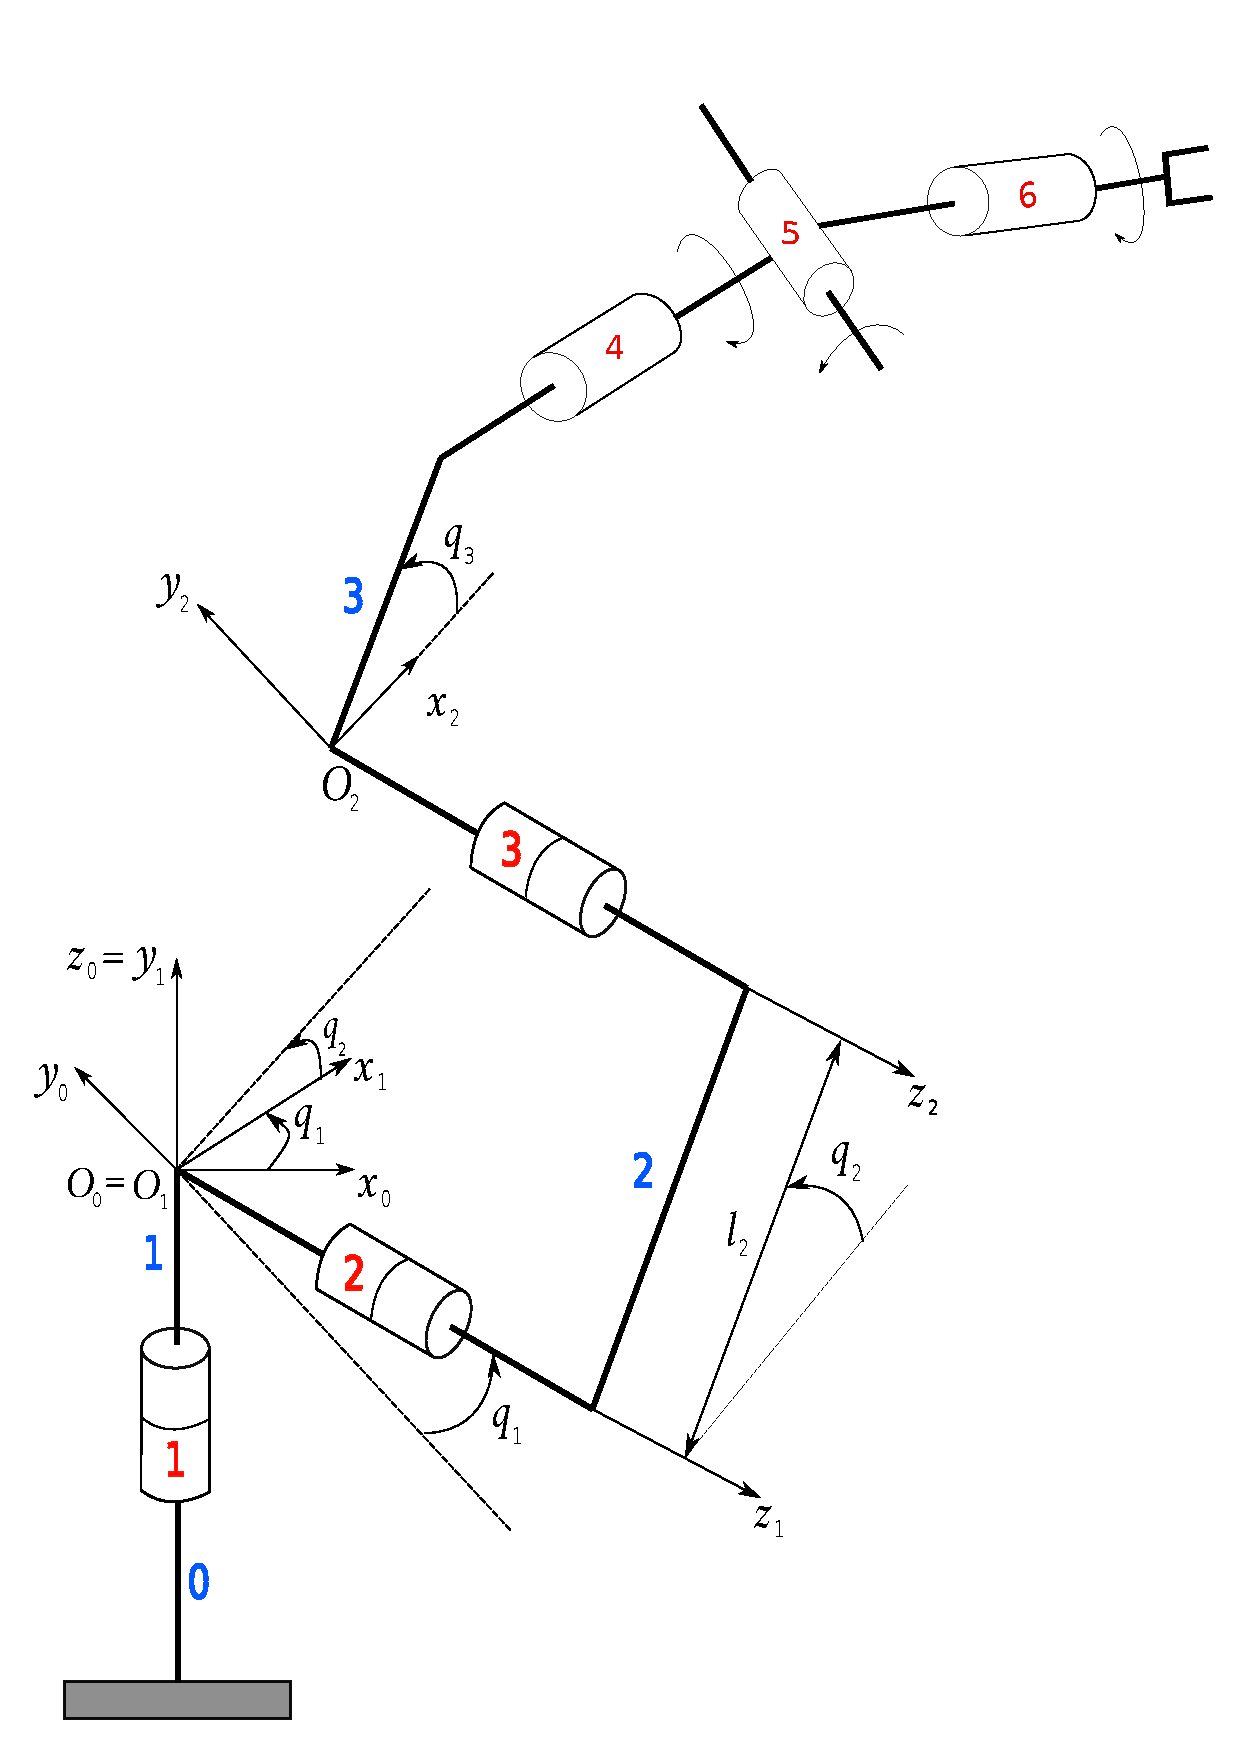
\includegraphics[scale=0.4]{manipolatoreCompleto.pdf}
\captionof{figure}{Manipolatore antropomorfo completo.}
\end{center}